\documentclass{standalone}
\usepackage{tikz}
\usetikzlibrary{shapes, arrows.meta, positioning, calc, fit, backgrounds}

\begin{document}
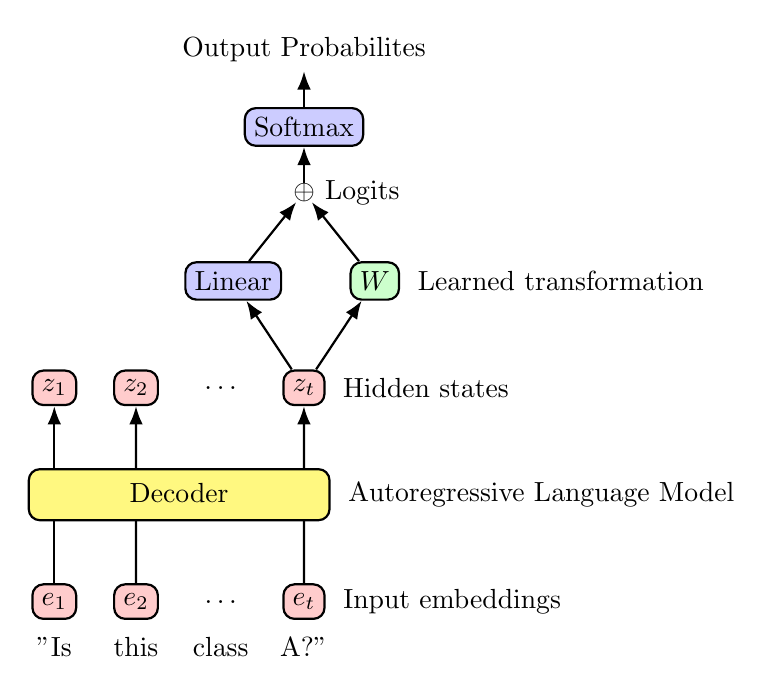
\begin{tikzpicture}[
    node distance=1cm and 1cm,
    mynode/.style={draw, thick, rounded corners, align=center},
    myarrow/.style={-Latex, thick},
    myblue/.style={fill=blue!20},
    myyellow/.style={fill=yellow!50},
    myred/.style={fill=red!20},
    mygreen/.style={fill=green!20},
]

% Define layers
\pgfdeclarelayer{background}
\pgfsetlayers{background,main}


% Nodes
\node[mynode, myred] (e1) {$e_1$};
\node[mynode, myred, right=3ex of e1] (e2) {$e_2$};
\node[right=3ex of e2] (edots) {$\dots$};
\node[mynode, myred, right=3ex of edots] (et) {$e_t$};

% text nodes
\node[below=0.1cm of e1] {"Is};
\node[below=0.1cm of e2]{this};
\node[below=0.19cm of edots] {class};
\node[below=0.1cm of et] {A?"};

\node[above=of e1] (d1) {};
\node[above=of et] (dt) {};
\node[mynode, myyellow, fit={(d1)(dt)}, inner sep=2mm, text height=1.5ex] (decoder) {Decoder};

\node[mynode, myred, above=of d1] (z1) {$z_1$};
\node[mynode, myred, right=3ex of z1] (z2) {$z_2$};
\node[right=3ex of z2] (zdots) {$\dots$};
\node[mynode, myred, right=3ex of zdots] (zt) {$z_t$};

\node[above=of zt] (linear_middle) {};
\node[mynode, myblue, left=1ex of linear_middle] (linear) {Linear};
\node[mynode, mygreen, right=3ex of linear_middle] (new_linear) {$W$};

\node[label={right:Logits}, inner sep=0, above=of $(linear)!0.5!(new_linear)$] (sum) {$\oplus$};
\node[mynode, myblue, above=3ex of sum] (softmax) {Softmax};
\node[above=3ex of softmax] (probs) {Output Probabilites};

% Draw the arrows in the background layer
\begin{pgfonlayer}{background}
    \draw[myarrow] (e1) -- (z1);
    \draw[myarrow] (e2) -- (z2);
    \draw[myarrow] (et) -- (zt);
    \draw[myarrow] (zt) -- (linear);
    \draw[myarrow] (zt) -- (new_linear);
    \draw[myarrow] (linear) -- (sum);
    \draw[myarrow] (new_linear) -- (sum);
    \draw[myarrow] (sum) -- (softmax);
    \draw[myarrow] (softmax) -- (probs);
\end{pgfonlayer}

% Labels
\node[right=0.1cm of new_linear] (l_W) {Learned transformation};
\node[right=0.1cm of zt] {Hidden states};
\node[right=0.1cm of decoder] {Autoregressive Language Model};
\node[right=0.1cm of et] {Input embeddings};

\end{tikzpicture}
\end{document}
